\PassOptionsToPackage{unicode=true}{hyperref} % options for packages loaded elsewhere
\PassOptionsToPackage{hyphens}{url}
%
\documentclass[]{article}
\usepackage[fontset=ubuntu]{ctex}
\usepackage{lmodern}
\usepackage{amssymb,amsmath}
\usepackage{ifxetex,ifluatex}
\usepackage{fixltx2e} % provides \textsubscript
\ifnum 0\ifxetex 1\fi\ifluatex 1\fi=0 % if pdftex
  \usepackage[T1]{fontenc}
  \usepackage[utf8]{inputenc}
  \usepackage{textcomp} % provides euro and other symbols
\else % if luatex or xelatex
  \usepackage{unicode-math}
  \defaultfontfeatures{Ligatures=TeX,Scale=MatchLowercase}
\fi
% use upquote if available, for straight quotes in verbatim environments
\IfFileExists{upquote.sty}{\usepackage{upquote}}{}
% use microtype if available
\IfFileExists{microtype.sty}{%
\usepackage[]{microtype}
\UseMicrotypeSet[protrusion]{basicmath} % disable protrusion for tt fonts
}{}
\IfFileExists{parskip.sty}{%
\usepackage{parskip}
}{% else
\setlength{\parindent}{0pt}
\setlength{\parskip}{6pt plus 2pt minus 1pt}
}
\usepackage{hyperref}
\hypersetup{
            pdfborder={0 0 0},
            breaklinks=true}
\urlstyle{same}  % don't use monospace font for urls
\setlength{\emergencystretch}{3em}  % prevent overfull lines
\providecommand{\tightlist}{%
  \setlength{\itemsep}{0pt}\setlength{\parskip}{0pt}}
\setcounter{secnumdepth}{0}
% Redefines (sub)paragraphs to behave more like sections
\ifx\paragraph\undefined\else
\let\oldparagraph\paragraph
\renewcommand{\paragraph}[1]{\oldparagraph{#1}\mbox{}}
\fi
\ifx\subparagraph\undefined\else
\let\oldsubparagraph\subparagraph
\renewcommand{\subparagraph}[1]{\oldsubparagraph{#1}\mbox{}}
\fi
\usepackage{graphicx, subfigure}
% set default figure placement to htbp
\makeatletter
\def\fps@figure{htbp}
\makeatother
\title{第二次作业}
\author{BobAnkh}

\date{}

\begin{document}

\maketitle

\hypertarget{header-n80}{%
\subsection{1.	零摄氏度空气中声速为331$m/s$,空气密度为1.293$kg/m^3$,其中一声波的声压级为74$dB$,试求其声压有效幅值,声强级别及声强的有效幅值,和平均声能量密度。}\label{header-n80}}

由题意可知,声压级$SPL=74dB$,由声压级和声压有效值的公式,可得:

\textbf{声压有效幅值}为:$p_e=p_{ref}10^{\frac{SPL}{20}}=2\times 10^{-5}\times 10^{\frac{74}{20}}=0.100Pa$

\textbf{声强级别}可以根据公式进行计算:$SIL=SPL+10\lg\frac{400}{\rho_0c_0}=74+10\lg \frac{400}{1.294\times 331}=73.71dB$

\textbf{声强的有效幅值}:$I_e=I_{ref}10^{\frac{SIL}{10}}=10^{-12}10^{\frac{73.71}{10}}=2.35\times 10^{-5}W/m^2$

\textbf{平均声能量密度}:$\bar{\epsilon}=\frac{I_e}{c_0}=\frac{2.35\times 10^{-5}}{331}=7.10\times 10^{-8} J/m^3$

\hypertarget{header-n87}{%
\subsection{2. 振幅较小的两列声波叠加后的声场的声压等于两列声波各自声压的和(声波叠加原理),已知两列小振幅声波叠加之后的声压级为$L$, 而两列声波声压级之差为Δ$L$, 求两列声波各自的声压。}\label{header-n87}}

设两列声波的声压分别为$p_{e1}$和$p_{e2}$,不妨设$p_{e1}<p_{e2}$,记两者的声压级分别为$L_1$和$L_2$则有:

$$L_1=20\lg\frac{p_{e1}}{p_{ref}}$$
$$L_2=20\lg\frac{p_{e2}}{p_{ref}}$$

根据题设条件有:

$$\begin{cases}L=20\lg\frac{p_{e1}+p_{e2}}{p_{ref}} \\ \Delta L=L_1-L_2=20\lg\frac{p_{e1}}{p_{e2}}\end{cases}$$

由此可以解得两列声波的声压:

$$p_{e1}=p_{ref}\frac{10^{\frac{L+\Delta L}{20}}}{1+10^{\frac{\Delta L}{20}}}$$
$$p_{e2}=p_{ref}\frac{10^{\frac{L}{20}}}{1+10^{\frac{\Delta L}{20}}}$$

\hypertarget{header-n94}{%
\subsection{3.	下图是一段浊音信号的时域波形(a)及其频谱(b),采样频率16000 $Hz$,从图(a)中分别用151点的Hamming窗(粗线)和501点的Hamming窗(细线)分别取出信号片段并计算其频谱,得到结果分别如图(b)中的粗线和细线所示。请根据这两幅图或其中的一幅估计语音信号的基音频率(F0)和第一共振峰频率(F1)。}\label{header-n94}}

\centerline{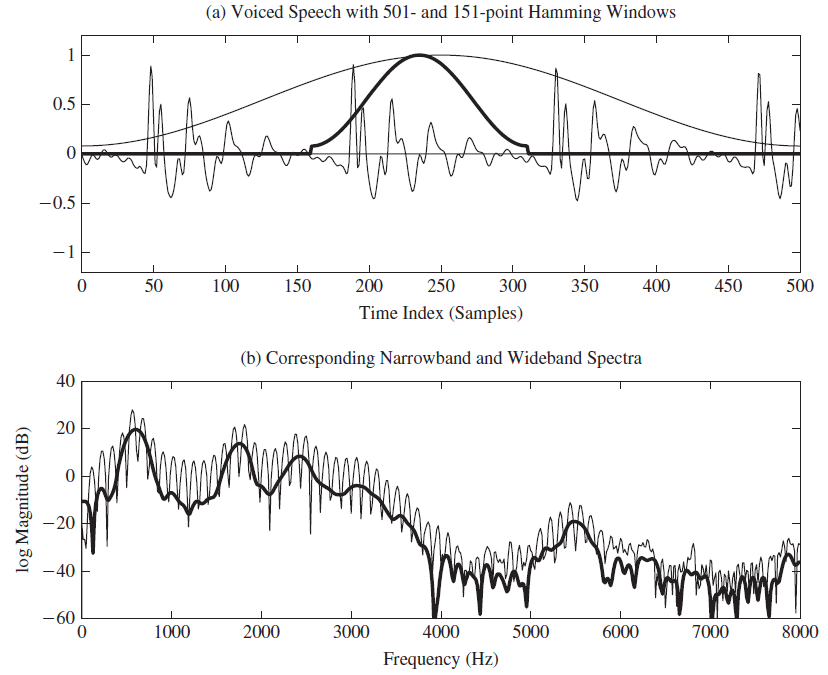
\includegraphics[scale=.75]{figures/q3.png}}

\textbf{估计基音频率($F_0$):}

可以看到第一张时域波形图中,包含了3个基音周期,一共涵盖了约425个点($50\rightarrow 475$),故一个基音周期平均就涵盖了141个点,由此可以计算基音周期:

$$P=\frac{141}{f_s}=8.8125\times 10^{-3}\;s$$

进而得到基音频率:

$$F_0=\frac{1}{P}=113.48\;Hz$$

\textbf{估计第一共振峰频率($F_1$):}

根据第二张频域图像,可以估计第一个峰的频率,也就是第一共振峰频率,约为:

$$F_1=600\;Hz$$

\hypertarget{header-n102}{%
\subsection{4.总结人类听觉系统对于声音方向辨别的主要原理和特点。}\label{header-n102}}

\textbf{主要原理}:

\begin{enumerate}
\def\labelenumi{\arabic{enumi}.}
\item
  双耳线索,即双耳间时间差ITD和双耳强度差ILD。当声源发出声音的时候,由于声源到两耳的距离一般不相等,因而声波传到人的两耳时会有时间差,而由于人头部自身对声音会有屏蔽阻挡,因而声波传到两耳时会有强度差,由此可以根据ITD和ILD进行声音方向的辨别。
\end{enumerate}

\begin{enumerate}
\def\labelenumi{\arabic{enumi}.}
\item
  单耳线索,即头部相关传输函数(Head Related Transfer
  Function),耳和头的构造会对声音产生滤波效果,因此鼓膜接收的声音频谱与音源的位置相关,不同的人会有不同的HRTF,从而进行定位。
\end{enumerate}

\textbf{特点}:

\begin{enumerate}
\def\labelenumi{\arabic{enumi}.}
\item
  人类的听觉定位精度与音源方位有关,前方的定位精度最高(2-3.5度),而后方的相对定位精度就差一些了(20度)。
\item
  ITD是低频音源位置判断的主要依据;ILD随着声音频率的增加而增大,因此是高频音源位置判断的主要依据;HRTF是声源落在同一个俯仰轴上时主要的位置判断依据
\item
  存在混淆椎体(con of
  confusion),即人在此椎体中的声音产生的ITD和ILD相同,所以需要单耳线索即HRTF来帮助定位
\end{enumerate}

\hypertarget{header-n104}{%
\subsection{5.简述听觉掩蔽效应在音频编码中的应用。}\label{header-n104}}

只需要对音频频谱大于掩蔽阈值的部分进行编码,低于阈值的部分被掩蔽而不需要编码

\hypertarget{header-n106}{%
\subsection{6.列举几种历史上出现过的有代表性的语音合成方法。}\label{header-n106}}

声码器,发音器官语音合成方法,单词拼接合成,单元选择方法,基于深度学习的端到端语音合成方法

\hypertarget{header-n108}{%
\subsection{7.简述语音识别的Bayesian原理,以及识别解码过程的三个步骤。}\label{header-n108}}

ASR问题通常被看作一个统计决策问题,它是一个Bayes最大后验概率(MAP)决策过程:

\begin{itemize}
\item
  给定一个特征向量序列$X$,(在任务语言中)寻找最大化后验概率$P(W|X)$的词串$\hat{W}$,即
\end{itemize}

$$\hat{W}=arg\max_WP(W|X)$$

\begin{itemize}
\item
  采用Bayes准则,可以重新写为如下形式:
\end{itemize}

$$\hat{W}=arg\max_W\frac{P(X|W)P(W)}{P(X)}$$

识别解码过程通常可以写为如下的三个步骤:

$$\hat{W}=\underbrace{arg\max_W}_{Step3}\underbrace{P_A(X|W)}_{Step1}\underbrace{P_L(W)}_{Step2}$$

\begin{itemize}
\item
  第一步是计算由句子$W$对应该语音的声学模型概率;
\item
  第二步是计算句子中词语的语言模型分数;
\item
  第三步是搜索任务语言中所有可能的句子,以得到最大似然的识别结果。
\end{itemize}

\end{document}
